\documentclass[final,hyperref={pdfpagelabels=false}]{beamer}
\mode<presentation>{\usetheme{Wernecke_bright}}
\usepackage[orientation=portrait,size=a0,scale=1.4,debug]{beamerposter}
\usepackage[english]{babel}
\usepackage[utf8]{inputenc}
\graphicspath{{./images/}}
\usepackage{wrapfig}


\usepackage[caption=false]{subfig}

\setbeamertemplate{caption}[numbered]
% packages and settings %%%%%%%%%%%%%%%%%%%%%%%%%%%%%%%%%%%%%%%%%%%%%%%%%%%%%%%%%%%%%%
% \usepackage{grffile}
\boldmath	

% PDF and title settings %%%%%%%%%%%%%%%%%%%%%%%%%%%%%%%%%%%%%%%%%%%%%%%%%%%%%%%%%%%%%
\title{Clique encoding in recurrent neural networks} %\\[0.2\baselineskip]with a second line
\author[varriale@itp.uni-frankfurt.de]{Emanuele Varriale, Claudius Gros}
\institute{Institute for Theoretical Physics, Goethe University, Frankfurt am Main, Germany}
\date{27$^\text{th}$ September 2018}
 
%%%%%%%%%%%%%%%%%%%%%%%%%%%%%%%%%%%%%%%%%%%%%%%%%%%%%%%%%%%%%%%%%%%%%%%%%%%%%%%%%%%%%%

\begin{document}

\begin{frame}
\hfill
\begin{columns}
	
	% ---------------------------------------------------------%
	% Set up a column 1
	\hfill
	\begin{column}{.30\textwidth}
		%\begin{beamercolorbox}[center,wd=\textwidth]{postercolumn}
		\begin{minipage}[T]{.95\textwidth}	% tweaks the width, makes a new \textwidth
		\parbox[t][\columnheight]{\textwidth}{

			%%% CONTENT of column 1 %%%
			%\vfill
			\begin{block}{Introduction}
			\begin{itemize}
					\item Internal brain activity is only modulated, not driven, by sensory input \cite{fiser2004modulation}. 
					
					\item Semantic learning has to result from the interaction of sensory stimuli with an autonomously active network.
					
					\item Clique encoding \cite{lin2006clique} can be achieved with a network of competing cliques, that has transient state dynamics.
										
					\item We propose a learning rule that correlates such transient states with sensory inputs from the bars and stripes problem, prompted by \cite{gros2010semantic}.
			\end{itemize}

			\end{block}
			
			\vfil
			\begin{block}{Network architecture}
				\begin{itemize}
					\item A clique is a maximal fully connected sub-graphs. 
					
					\item Cliques compete with one another if they have predominantly inhibitory connections across and excitatory ones within.
					
					\item A single active clique is a stable state, as long as other cliques are inhibited.
				\end{itemize}
			
			\begin{figure}
				\centering
				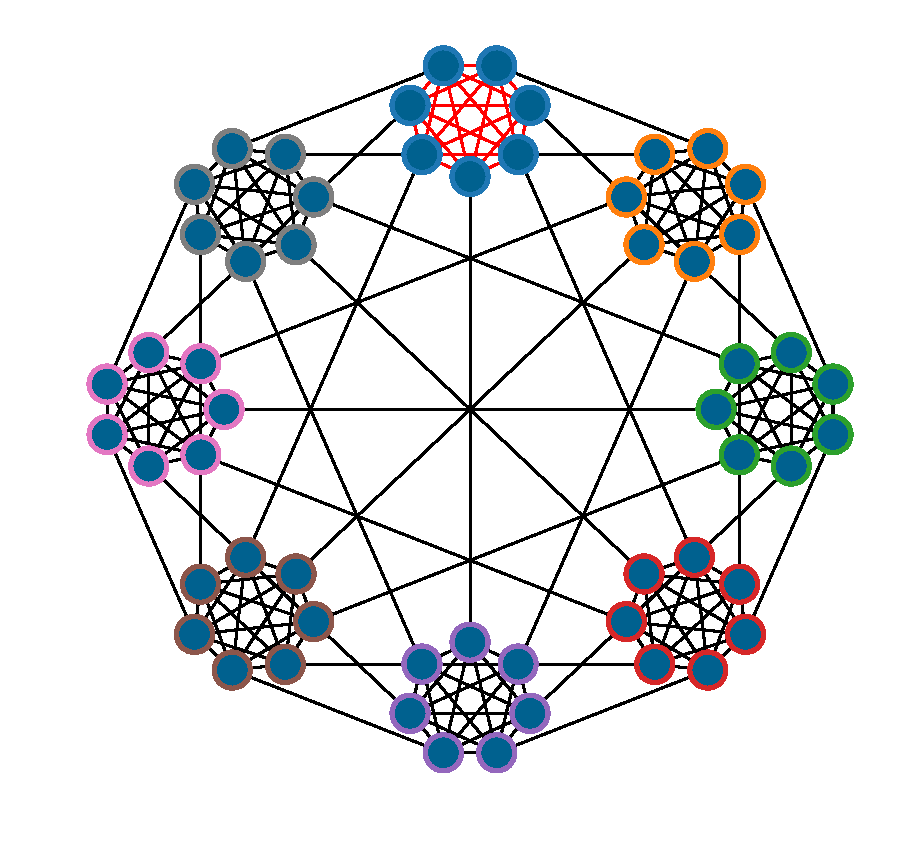
\includegraphics[width=.8\linewidth]{network2.pdf}
				\caption{An eight clique network, each with seven nodes. Only excitatory links are shown. Each neuron within a clique excites an extra-clique neuron. The network is completed with inhibitory connections.}
				\label{fig:network}
			\end{figure}
			\end{block}		
							
			\vfil
			\begin{block}{Neuronal dynamics}
				\begin{itemize}
					\item A rate-encoding model is used.
					\item The $j$-th neuron has membrane potential $x_j$, activity $y_j$ and excitatory and inhibitory input, $E_j$ and $I_j$.
				\end{itemize}
			\begin{gather*}
				\tau_x \dot{x}_j = -x_j + E_j + I_j\\
				y_j = \sigma \left(x_j\right) = \frac{1}{1+\exp \left(-a x_j \right) } \\
				E_j = \sum_{k} w_{jk} y_k \\
				I_j = \sum_k z_{jk} y_k.
				\label{eq:neuron}
			\end{gather*}
			\begin{itemize}
				\item With these equation the system rapidly relaxes to a stable active clique state.
				
				\item The inclusion of presynaptic short-term plasticity, transforming $y_k \rightarrow \tilde{y}_k$, gives transient state dynamics, as in Fig. \ref{fig:activity}.
			\end{itemize}		
		
				\begin{figure}
					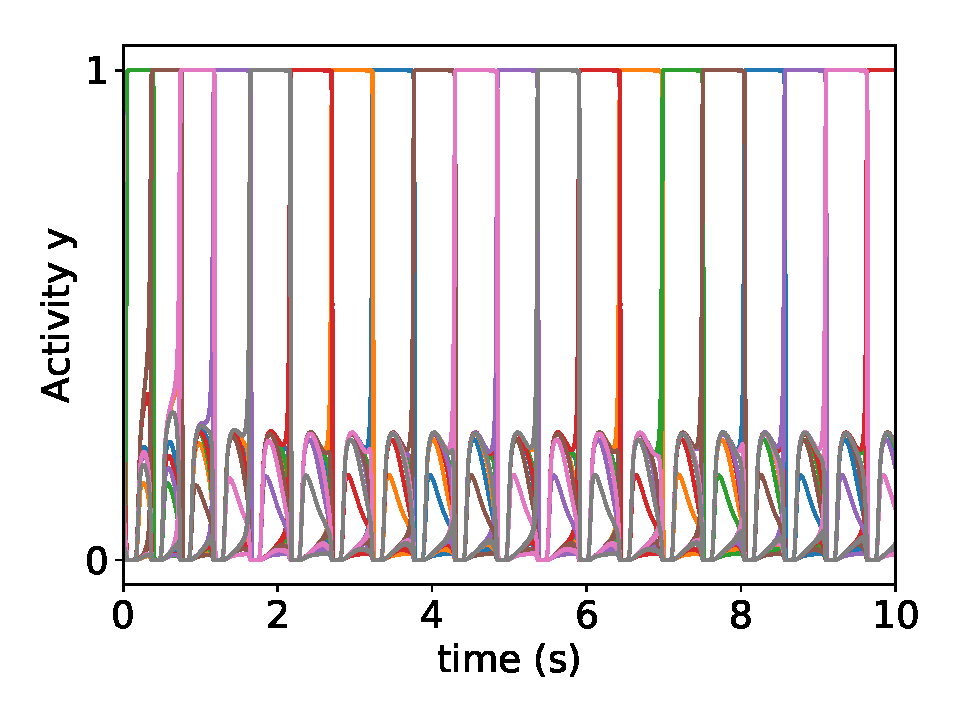
\includegraphics[width=.8\linewidth]{double_activity}
					\caption{Internal activity in the network shown above, with the full depletion model.Neurons belonging to the same clique share plotting colours, as in Fig. \ref{fig:network}.}
					\label{fig:activity}
				\end{figure}
		

			
			\end{block}
			\vfil
			\begin{refblock}{References}

					\begin{thebibliography}{1}

						\bibitem{fiser2004modulation}
						Fiser, J., Chiu, C. \& Weliky, M. Small modulation of ongoing cortical dynamics by sensory input during natural vision. Nature 431, 573 (2004).
						
						
						\bibitem{lin2006clique} Lin, L., Osan, R. \& Tsien, J. Z. Organizing principles of real-time memory encoding: neural clique assemblies and universal neural codes. Trends in Neurosciences 29, 48–57 (2006).
						
						\bibitem{gros2010semantic}
						Gros, C. \& Kaczor, G. Semantic learning in autonomously active recurrent neural networks. Log J IGPL 18, 686–704 (2010).
						
						\bibitem{tsodyks2008model}
						Mongillo, G., Barak, O. \& Tsodyks, M. Synaptic Theory of Working Memory. Science 319, 1543–1546 (2008).

					\end{thebibliography}

			\end{refblock}
			%\vfil
			%%% END CONTENT of column 1 %%%

	 	} % end of parbox
		\end{minipage}
		%\end{beamercolorbox}
	\end{column}
	% ---------------------------------------------------------%
	% end of column 1
	\hfil
	% ---------------------------------------------------------%
	% Set up a column 2
	\begin{column}{.60\textwidth}
		%\begin{beamercolorbox}[center,wd=\textwidth]{postercolumn}
		\begin{minipage}[T]{.95\textwidth}
		\parbox[t][\columnheight]{\textwidth}{
		%%% CONTENT of column 2 %%%
		\vfil
		\begin{block}{Full depletion model}
			\begin{columns}
				\begin{column}[T]{.4\textwidth}
				\begin{figure}
					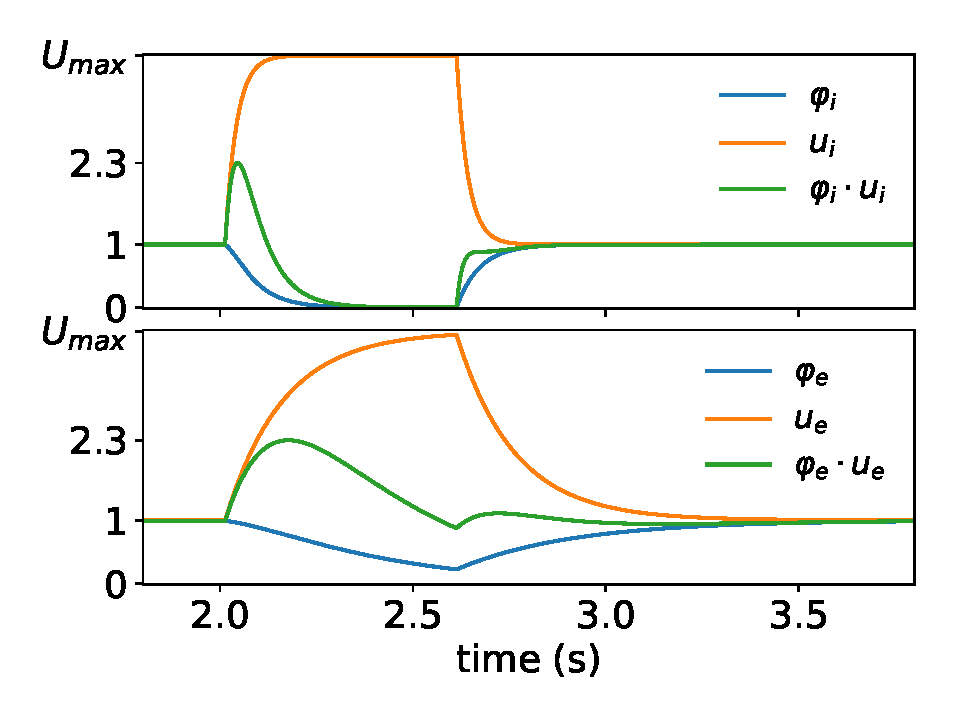
\includegraphics[width=.9\linewidth]{double_depletion_big.pdf}
					\caption{Dynamics of the full depletion model, with high presynaptic activity, for inhibitory (top) and excitatory (bottom) synapses.}
					\label{fig:full_depletion}
				\end{figure}
				\end{column}							
				\begin{column}[T]{.6\textwidth}
					\begin{itemize}
						\item Winning clique states become unstable with the STP \emph{full depletion model}, that is inspired by the Tsodyks-Markram model \cite{tsodyks2008model}.
						
						\item Transient states are obtained by modelling neurotransmitter vesicles with: 
						\begin{itemize}
							\item $u_k$: likelihood of neurotransmitter release, increases with input						
							\item $\varphi_k$: concentration of vesicles, that deplete while firing.
						\end{itemize}
						
						\item Inhibitory synapses deplete faster than excitatory ones.
					\end{itemize}
					\begin{gather*}
						y_k \rightarrow \tilde{y}_k = y_k u_k \varphi_k \\
						\dot{u}_k = \frac{U_y -u_k}{T_u}, \quad U_y = 1 + \left( U_\text{max} -1 \right) y_k\\ 
						\dot{\varphi}_k = \frac{\varPhi_u - \varphi_k}{T_\varphi}, \quad \varPhi_u = 1- \frac{u_k y_k}{U_\text{max}} \\
						T^{\text{exc}} = 5 \cdot T^{\text{inh}}.
					\end{gather*}
				\end{column}
			\end{columns}
		\end{block}
		\vfil
			\begin{block}{Sensory input}
				\begin{columns}
					\begin{column}[T]{.55\textwidth}		
						\begin{itemize}
							\item Cognitive systems must identify objects in a noisy environment, performing independent component analysis.
							
							\item Sensory input consists of vertical and horizontal bars
							presented on a retina of $L \times L$ pixels
							
							\item Each bar is independently drawn with probability $p=1/2L$.
							
							\item Inactive pixels have output $y_l^{\text{ext}}=0$, and active pixels $y_l^{\text{ext}}=1$, even at the intersection of two bars.
							
							\item Therefore, \emph{non linear} independent component analysis has to be performed to separate bars.
							
							\item At regular intervals, the all-to-all sensory connections transmit the extra excitatory input
								\begin{equation*}
								\Delta E_j = \sum_{l} v_{jl} y_l^{\text{ext}}
								\end{equation*}
						\end{itemize}						
					\end{column}
					\begin{column}[T]{.45\textwidth}	
						\begin{figure}[T]
							\subfloat[Activity with sensory input shown by vertical stripes.]{%
								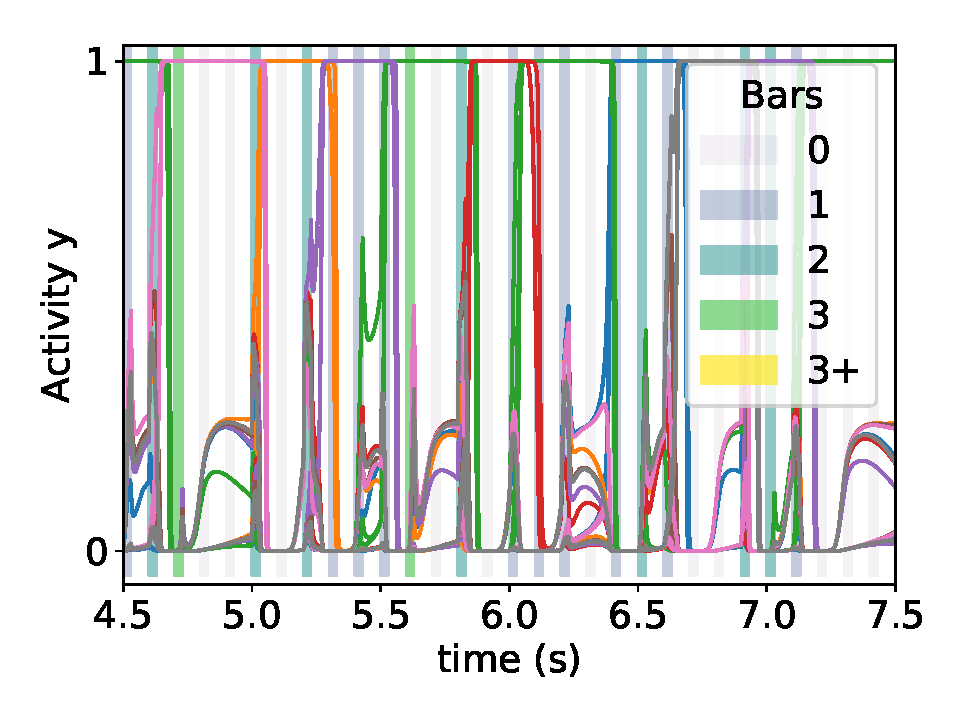
\includegraphics[clip,width=.9\textwidth]{double_sens_activity2.pdf}%
							}
							
							\subfloat[Examples of input patterns.]{%
								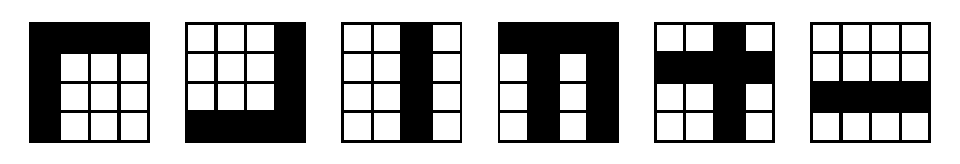
\includegraphics[clip,width=0.8\textwidth]{input_ex6.pdf}%
							}
							%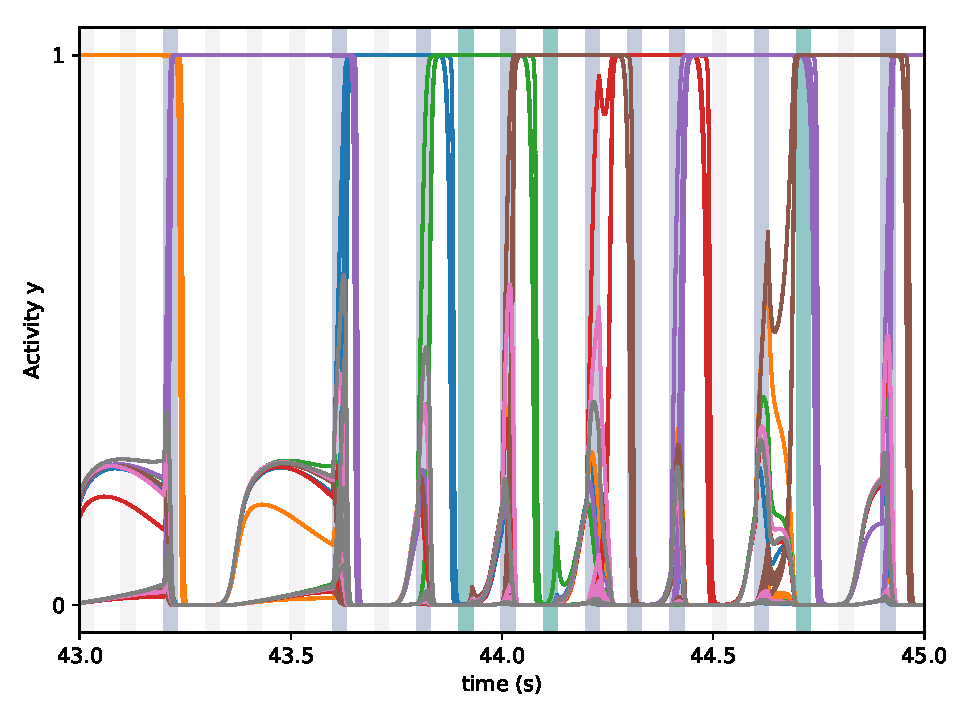
\includegraphics[width=1\textwidth]{double_sens_activity.pdf}
							%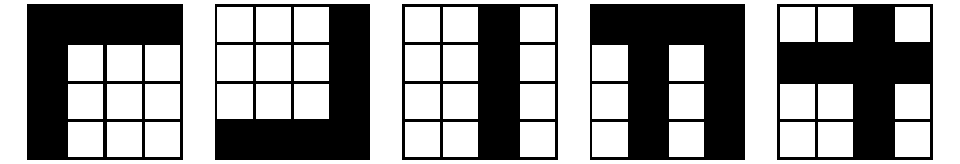
\includegraphics[width=1\textwidth]{input_ex.pdf}	
						\end{figure}
					\end{column}
				\end{columns}
			\end{block}
			\vfil
			\begin{minipage}[T]{.55\textwidth}
			\begin{block}{Learning rule}
				
				\begin{columns}
					\begin{column}[T]{1\textwidth}
						\begin{itemize}
							\item The sensory weights $v_{jl}$ must change so that different cliques respond mostly to single different bars.
							
							\item We hypothesize that learning occurs during the transitions from one winning clique to another.
						\end{itemize}
						\begin{gather*}
						\dot{v}_{jl} = \left(\dot{y}_j c_j / \tau_v  - 1 / \tau_d\right) y_l^{\text{ext}} v_{jl}  \\
						c_j = \tanh{\left[a \left(V_t - \Delta E_j \right)\right]} \\
						V_t = V^{\text{inact}} + y_j \left(V^{\text{act}} - V^{\text{inact}}\right)\\
						\tau_v \ll \tau_d, \quad V^{\text{inact}} < V^{\text{act}}.	
						\end{gather*}
						\begin{itemize}
							\item $v_{jl}$ ensures that the weights do not change sign,
							\item sensory input $y_l^{\text{ext}}$ is necessary,
							\item $\dot{y}_j = 0$ during winning clique states,
							\item $c_j$ prevents runaway synapses dynamics, through the sliding activity level target $V_t$,
							\item the slow decay term $-1/\tau_d$ shrinks orthogonal synapses.
						\end{itemize}
					\end{column}
			
				\end{columns}
			\end{block}
		%\end{minipage}
		\vfill
		%	\begin{minipage}[T]{.5\textwidth}
			\begin{block}{Results}
				\begin{columns}									
					\begin{column}[T]{1\textwidth}
						We use two performance measures:
						\begin{gather*}
						R(\alpha, \beta) = \frac{1}{S_\alpha} \sum_{\substack{i\in C_\alpha \\ l \in P_\beta}} v_{il} y_l^{\text{ext}} \\
						F(\alpha, l) = \frac{1}{S_\alpha} \sum_{i\in C_\alpha} v_{il}
						\end{gather*}
						\begin{itemize}
							\item The response $R(\alpha, \beta)$ is the clique averaged input received by clique $\alpha$ of size $S_\alpha$, when bar $\beta$ is active.
							
							\item Ideally, $R(\alpha, \beta)$ would have a single maximum, that would be different across cliques.
							
							\item The receptive field $F(\alpha, l)$ is the clique averaged sensory synaptic weight from the $j$-th pixel.
							
							\item Ideally, $F(\alpha, l)$ would mirror the input from the most important bar.
						\end{itemize}
						
					\end{column}
					
				\end{columns}
			\end{block}
			\end{minipage}			
			\begin{minipage}[T]{.45\textwidth}
				\vspace{1\baselineskip}
				\begin{column}[T]{1\textwidth}
					\begin{figure}
						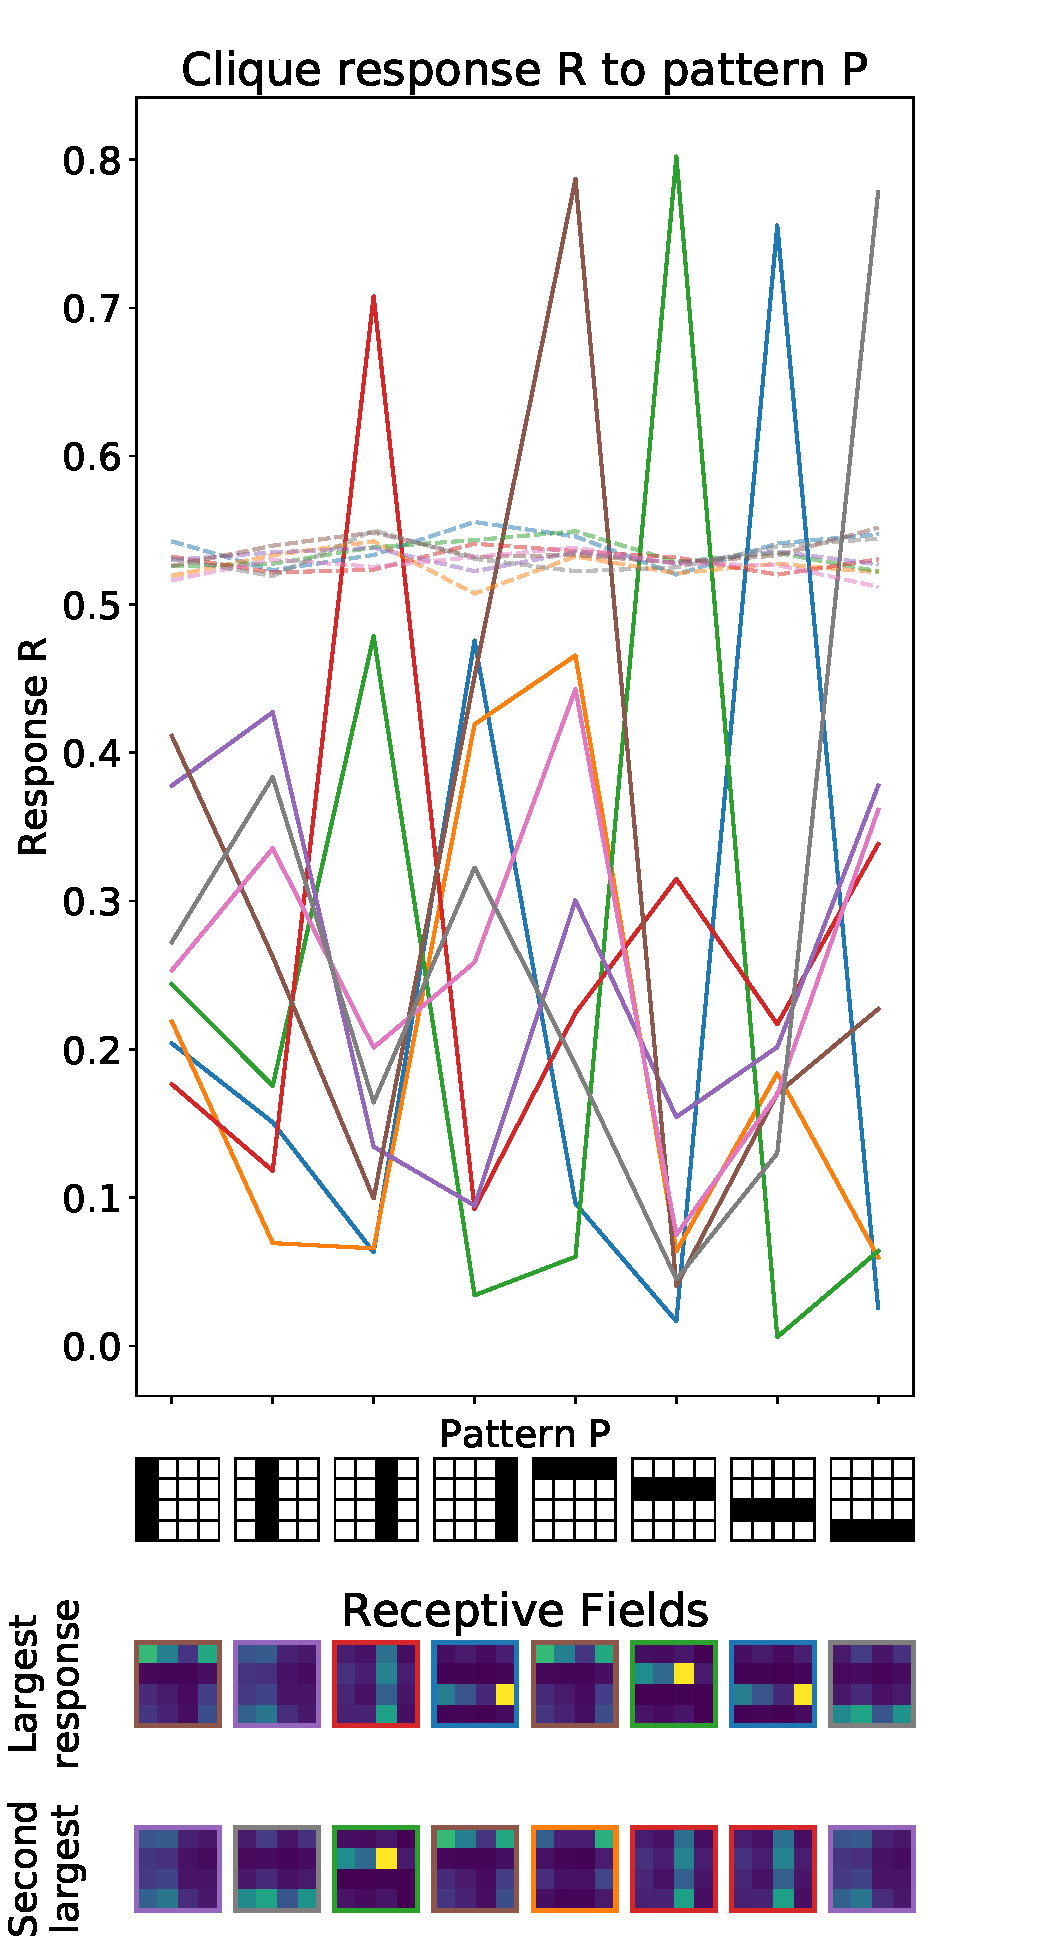
\includegraphics[width=.89\textwidth]{double_complete_tall.pdf}
						\caption{{\color{black}Performance of the learning rule. Top: clique response for every bar, dashed lines show initial responses. Bottom: receptive fields of the two cliques that respond the most to given patterns. The colour coding increases from violet	to yellow.}}
						\label{fig:complete}
					\end{figure}
				\end{column}
			\end{minipage}
			\vfill
			\vspace{1\baselineskip}
			\begin{emphblock}{Conclusions}
				\singleitem{In neural networks designed for feature extraction activity usually dies out without input. This is not, however, how actual brains operate.}
				\singleitem{This work is a proof of concept showing how feature extraction with an autonomously active network can be achieved.}
				\singleitem{Internal activity is characterized by transient states and competitive dynamics, and learning occurs during transitions between active cliques.}
				\singleitem{More work is needed to improve performance and robustness of the algorithm.}
			\end{emphblock}

		\vfill

		%\vfil
		%%% END CONTENT of column 2 %%%


		} % end of parbox
		% ---------------------------------------------------------%
		% end the column
		\end{minipage}
		%\end{beamercolorbox}
	\end{column}
	\hfil
	% ---------------------------------------------------------%
	% end of column 2
\end{columns}
\hfill
\vfill
\vskip1ex
\end{frame}
\end{document}
